\documentclass[11pt]{article}

% ====================================================
% PACKAGES
% ====================================================
\usepackage[margin=1in, headheight=13.6pt]{geometry}
\usepackage[T1]{fontenc}
\usepackage{lmodern}
\usepackage{microtype}
\usepackage{setspace}
\usepackage{tcolorbox}
\usepackage{amsmath, amssymb, mathtools}
\usepackage{siunitx}

\usepackage{graphicx}
\usepackage{float}
\usepackage{subcaption}

\usepackage{enumitem}
\usepackage{booktabs}
\usepackage{longtable}
\usepackage{array}
\usepackage{multirow}

\usepackage{xcolor}
\usepackage{hyperref}

\usepackage{fancyhdr}
\usepackage{lastpage}

\usepackage{listings}
\usepackage{indentfirst}
\usepackage[justification=centering]{caption}

% Python source style for \CodeListing
\lstdefinestyle{pystyle}{
    language=Python,
    basicstyle=\ttfamily\footnotesize,
    keywordstyle=\color{blue!60!black}\bfseries,
    stringstyle=\color{orange!70!black},
    commentstyle=\color{gray!60!black}\itshape,
    numbers=left,
    numberstyle=\tiny\color{gray!70},
    numbersep=8pt,
    breaklines=true,
    showstringspaces=false,
    frame=single,
    rulecolor=\color{gray!40},
    tabsize=4,
    columns=fullflexible,
    captionpos=b,
    literate={°}{{\textdegree}}1,
}
\lstset{style=pystyle}

\pagestyle{fancy}
\fancyhf{}
\lhead{\Assignment\ |\ \course}
\rhead{\Name\ |\ \today}
\cfoot{Page \thepage\ of~\pageref{LastPage}}

\hypersetup{
    colorlinks,
    linkcolor={red!50!black},
    citecolor={blue!50!black},
    urlcolor={blue!80!black}
}

\newcommand{\Name}{Arael Anaya}
\newcommand{\Assignment}{Homework 7}
\newcommand{\course}{Advanced Dynamics}

% Boxed final-answer environment
\newtcolorbox{result}{
    colback=blue!3!white,
    colframe=blue!40!black,
    boxrule=0.6pt,
    arc=2pt,
    left=6pt, right=6pt, top=4pt, bottom=4pt
}

% Code listing: sources the .py file directly.
\newcommand{\CodeListing}[3]{%
\IfFileExists{#1}%
    {\lstinputlisting[style=pystyle,caption={#2},label={#3}]{#1}}%
    {\begin{quote}\itshape Source file \texttt{#1} not found yet --- this
        listing will populate automatically once the file is written.\end{quote}}}

\begin{document}

% ====================================================
% PROBLEM 1
% ====================================================
\section*{Problem 1}

\begin{figure}[H]
    \centering
    
\includegraphics[width=0.95\linewidth]{Figures/Problem Set/Problem 1.png}
\end{figure}

\subsection*{Part (a)}
Frame $\{d\}$ has the same orientation as $\{a\}$, so $R_{ad}=I$, and its offset can be read directly from the figure. Frame $\{d\}$ is also unrotated relative to $\{c\}$ up to the sign flip on $\hat z$, and its offset below $\{c\}$ is the height 2:
\[
T_{ad} = \begin{bmatrix} 1&0&0&-1\\0&1&0&1\\0&0&1&0\\0&0&0&1\end{bmatrix}, \qquad
T_{cd} = \begin{bmatrix} 0&1&0&0\\1&0&0&0\\0&0&-1&2\\0&0&0&1\end{bmatrix}
\]

\subsection*{Part (b)}
Frame $\{d\}$ is common to both the $\{a\}$-chain and the $\{b\}$-chain, so
\[
T_{ab} = T_{ad}\,T_{dc}\,T_{cb}
\]
where $T_{cb}=T_{bc}^{-1}$ and $T_{dc}=T_{cd}^{-1}$, using the rigid-body inverse $T^{-1}=\begin{bmatrix}R^T & -R^TP\\0^T&1\end{bmatrix}$:
\[
T_{cb} = \begin{bmatrix}1&0&0&-4\\0&1&0&0\\0&0&1&0\\0&0&0&1\end{bmatrix}, \qquad
T_{dc} = \begin{bmatrix}0&1&0&0\\1&0&0&0\\0&0&-1&2\\0&0&0&1\end{bmatrix}
\]
Multiplying $T_{dc}T_{cb}$ first,
\[
T_{dc}T_{cb} = \begin{bmatrix}0&1&0&0\\1&0&0&-4\\0&0&-1&2\\0&0&0&1\end{bmatrix}
\]
and then left-multiplying by $T_{ad}$ gives
\begin{result}
\[
T_{ab} = \begin{bmatrix}0&1&0&-1\\1&0&0&-3\\0&0&-1&2\\0&0&0&1\end{bmatrix}
\]
\end{result}


% ====================================================
% PROBLEM 2
% ====================================================
\newpage
\section*{Problem 2}

\begin{figure}[H]
    \centering
    
\includegraphics[width=0.95\linewidth]{Figures/Problem Set/Problem 2.png}
\end{figure}

With $\ell_0=\ell_1=\ell_2=1$, the zero-position end-effector configuration is
\[
M = \begin{bmatrix}1&0&0&0\\0&1&0&\ell_1+\ell_2\\0&0&1&\ell_0\\0&0&0&1\end{bmatrix}
  = \begin{bmatrix}1&0&0&0\\0&1&0&2\\0&0&1&1\\0&0&0&1\end{bmatrix}
\]

\subsection*{Screw Axes in \{0\}}
The first three joints are revolute about $\hat z_0$, each located along the $\hat x_0$ axis at increasing offset; the fourth is prismatic along $\hat z_0$:
\[
\mathcal S_1=\begin{pmatrix}0\\0\\1\\0\\0\\0\end{pmatrix},\quad
\mathcal S_2=\begin{pmatrix}0\\0\\1\\\ell_1\\0\\0\end{pmatrix}=\begin{pmatrix}0\\0\\1\\1\\0\\0\end{pmatrix},\quad
\mathcal S_3=\begin{pmatrix}0\\0\\1\\\ell_1+\ell_2\\0\\0\end{pmatrix}=\begin{pmatrix}0\\0\\1\\2\\0\\0\end{pmatrix},\quad
\mathcal S_4=\begin{pmatrix}0\\0\\0\\0\\0\\1\end{pmatrix}
\]
with matrix forms
\[
[\mathcal S_1]=\begin{bmatrix}0&-1&0&0\\1&0&0&0\\0&0&0&0\\0&0&0&0\end{bmatrix}, \qquad
[\mathcal S_2]=\begin{bmatrix}0&-1&0&1\\1&0&0&0\\0&0&0&0\\0&0&0&0\end{bmatrix}
\]
\[
[\mathcal S_3]=\begin{bmatrix}0&-1&0&2\\1&0&0&0\\0&0&0&0\\0&0&0&0\end{bmatrix}, \qquad
[\mathcal S_4]=\begin{bmatrix}0&0&0&0\\0&0&0&0\\0&0&0&1\\0&0&0&0\end{bmatrix}
\]

\subsection*{Spatial Form of the Product of Exponentials}
\[
T(\theta) = e^{[\mathcal S_1]\theta_1}\,e^{[\mathcal S_2]\theta_2}\,e^{[\mathcal S_3]\theta_3}\,e^{[\mathcal S_4]\theta_4}\,M
\]
with $e^{[\mathcal S]\theta}=\begin{bmatrix}e^{[\omega]\theta} & \big(I\theta+(1-\cos\theta)[\omega]+(\theta-\sin\theta)[\omega]^2\big)v\\0&1\end{bmatrix}$, $e^{[\omega]\theta}=I+\sin\theta[\omega]+(1-\cos\theta)[\omega]^2$, and $\theta=(0,\ \pi/2,\ -\pi/2,\ 1)$.

Since $\theta_1=0$, $e^{[\mathcal S_1]\theta_1}=I$. For $\theta_2=\pi/2$,
\[
e^{[\mathcal S_2]\pi/2} = \begin{bmatrix}0&-1&0&1\\1&0&0&1\\0&0&1&0\\0&0&0&1\end{bmatrix}
\]
For $\theta_3=-\pi/2$,
\[
e^{[\mathcal S_3](-\pi/2)} = \begin{bmatrix}0&1&0&-2\\-1&0&0&2\\0&0&1&0\\0&0&0&1\end{bmatrix}
\]
Joint 4 is prismatic, so $e^{[\mathcal S_4]\theta_4}$ is a pure translation by $v_4\theta_4$; with $\theta_4=1$,
\[
e^{[\mathcal S_4](1)} = \begin{bmatrix}1&0&0&0\\0&1&0&0\\0&0&1&1\\0&0&0&1\end{bmatrix}
\]
Multiplying the four exponentials with $M$ in order gives
\begin{result}
\[
T = \begin{bmatrix}1&0&0&-1\\0&1&0&1\\0&0&1&2\\0&0&0&1\end{bmatrix}
\]
\end{result}

\subsection*{Body Form Check}
The body screw axes are $\mathcal B_i = \mathrm{Ad}_{M^{-1}}\,\mathcal S_i$, where
\[
M^{-1} = \begin{bmatrix}1&0&0&0\\0&1&0&-2\\0&0&1&-1\\0&0&0&1\end{bmatrix}, \qquad
\mathrm{Ad}_{M^{-1}} = \begin{bmatrix}R&0\\ [p]R & R\end{bmatrix}
= \begin{bmatrix}1&0&0&0&0&0\\0&1&0&0&0&0\\0&0&1&0&0&0\\0&1&-2&1&0&0\\-1&0&0&0&1&0\\2&0&0&0&0&1\end{bmatrix}
\]
since $R=I$ for $M^{-1}$. This gives
\[
\mathcal B_1=\begin{pmatrix}0\\0\\1\\-2\\0\\0\end{pmatrix}, \quad
\mathcal B_2=\begin{pmatrix}0\\0\\1\\-1\\0\\0\end{pmatrix}, \quad
\mathcal B_3=\begin{pmatrix}0\\0\\1\\0\\0\\0\end{pmatrix}, \quad
\mathcal B_4=\begin{pmatrix}0\\0\\0\\0\\0\\1\end{pmatrix}
\]
Evaluating $T(\theta)=M\,e^{[\mathcal B_1]\theta_1}e^{[\mathcal B_2]\theta_2}e^{[\mathcal B_3]\theta_3}e^{[\mathcal B_4]\theta_4}$ with the same $\theta$ is guaranteed to reproduce the identical result, since $\mathcal B_i=\mathrm{Ad}_{M^{-1}}\mathcal S_i$ by construction:
\[
T = \begin{bmatrix}1&0&0&-1\\0&1&0&1\\0&0&1&2\\0&0&0&1\end{bmatrix}
\]


% ====================================================
% PROBLEM 4
% ====================================================
\newpage
\section*{Problem 3}

\begin{figure}[H]
    \centering
    
\includegraphics[width=0.95\linewidth]{Figures/Problem Set/Problem 3.png}
\end{figure}

\subsection*{Inverse Kinematics Derivation}
Subtracting off the last link along the desired tip orientation gives the wrist-center position, decoupling the problem into a planar 2R reach followed by an orientation adjustment:
\[
\vec\rho_w = \vec P_E - L_3\big(\cos\theta\,\hat x+\sin\theta\,\hat y\big)
\]
The $L_1$-$L_2$-$\rho_w$ triangle then gives $\beta$ by the law of cosines, and $\alpha$ from the angle between $L_1$ and $\rho_w$:
\[
L_1^2+L_2^2-2L_1L_2\cos\beta = |\rho_w|^2
\ \Longrightarrow\
\beta = \cos^{-1}\!\left(\frac{L_1^2+L_2^2-|\rho_w|^2}{2L_1L_2}\right)
\]
\[
\alpha = \cos^{-1}\!\left(\frac{|\rho_w|^2+L_1^2-L_2^2}{2L_1|\rho_w|}\right), \qquad \gamma = \operatorname{atan2}(\rho_w)
\]
and the joint angles follow directly:
\[
\theta_1 = \gamma-\alpha, \qquad \theta_2 = \pi-\beta, \qquad \theta_3 = \theta-\theta_1-\theta_2
\]
Taking $\beta\to-\beta$ (equivalently $\alpha\to-\alpha$) flips the elbow and produces the second branch, so every reachable pose has exactly two analytical solutions. Both branches are implemented in \texttt{Problem 3.py} (Appendix) and checked against the forward-kinematics map for each test case.

\subsection*{Results}
\begin{table}[H]
\centering
\begin{tabular}{c c c c c}
\toprule
State & Solution & $\theta_1$ [rad] & $\theta_2$ [rad] & $\theta_3$ [rad] \\
\midrule
\multirow{2}{*}{A: $(4,\ 0.5,\ 22^\circ)$} & 1 & $-0.6297$ & $1.8704$ & $-0.8568$ \\
 & 2 & $0.7113$ & $4.4128$ & $-4.7400$ \\
\midrule
\multirow{2}{*}{B: $(1.5,\ -1.5,\ -105^\circ)$} & 1 & $-1.0027$ & $2.5011$ & $-3.3309$ \\
 & 2 & $0.4131$ & $3.7821$ & $-6.0278$ \\
\bottomrule
\end{tabular}
\caption{Both analytical IK solutions for each test case; every row was confirmed to reproduce $(x,y,\theta)$ through the forward-kinematics map.}
\end{table}

\begin{figure}[H]
    \centering
    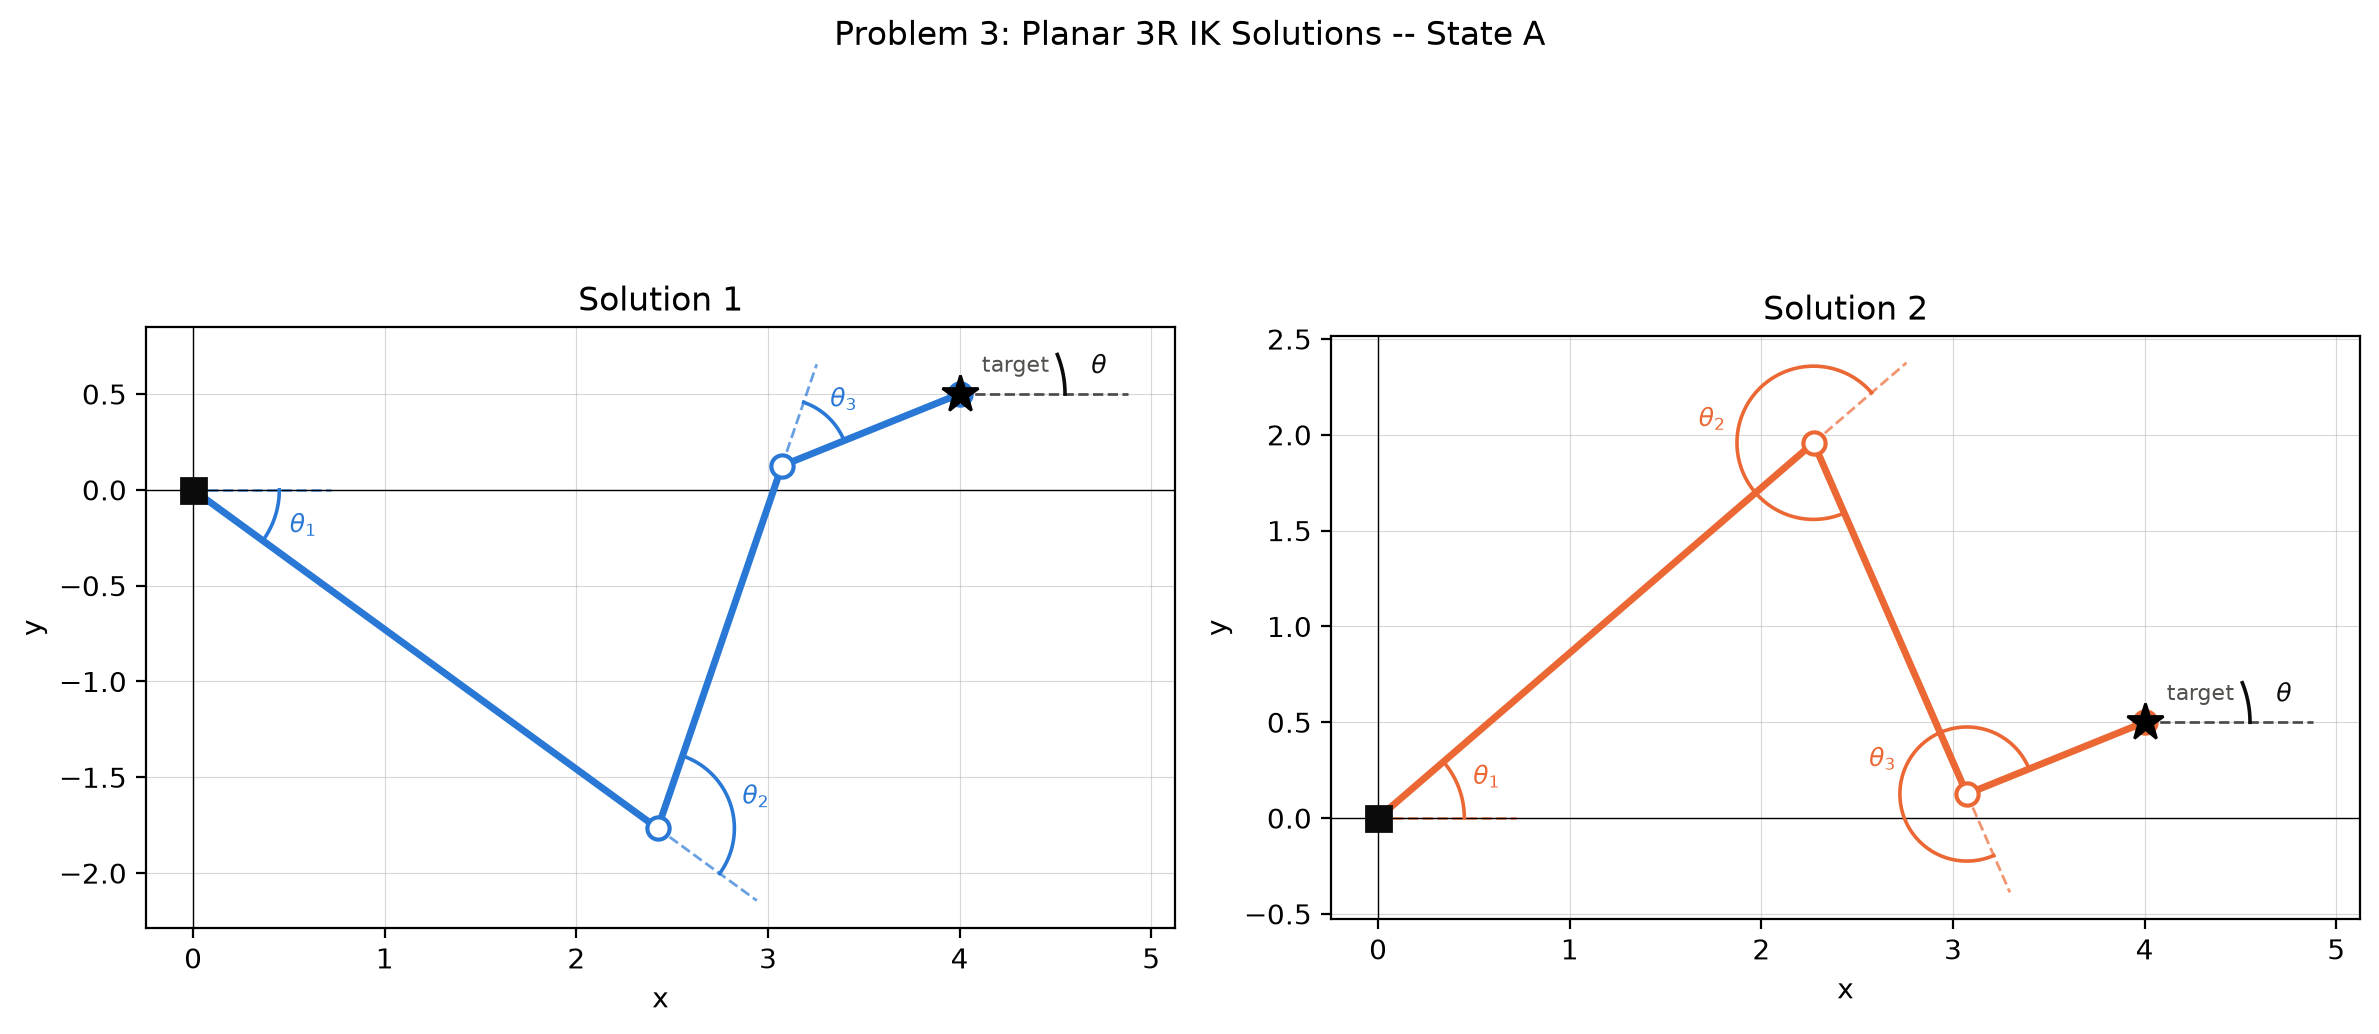
\includegraphics[width=\linewidth]{Figures/Graphs/Problem3_A.png}
    \caption{State A: $(x,y,\theta)=(4,\ 0.5,\ 22^\circ)$ -- elbow-up and elbow-down solutions, with joint angles marked at each joint.}
\end{figure}

\begin{figure}[H]
    \centering
    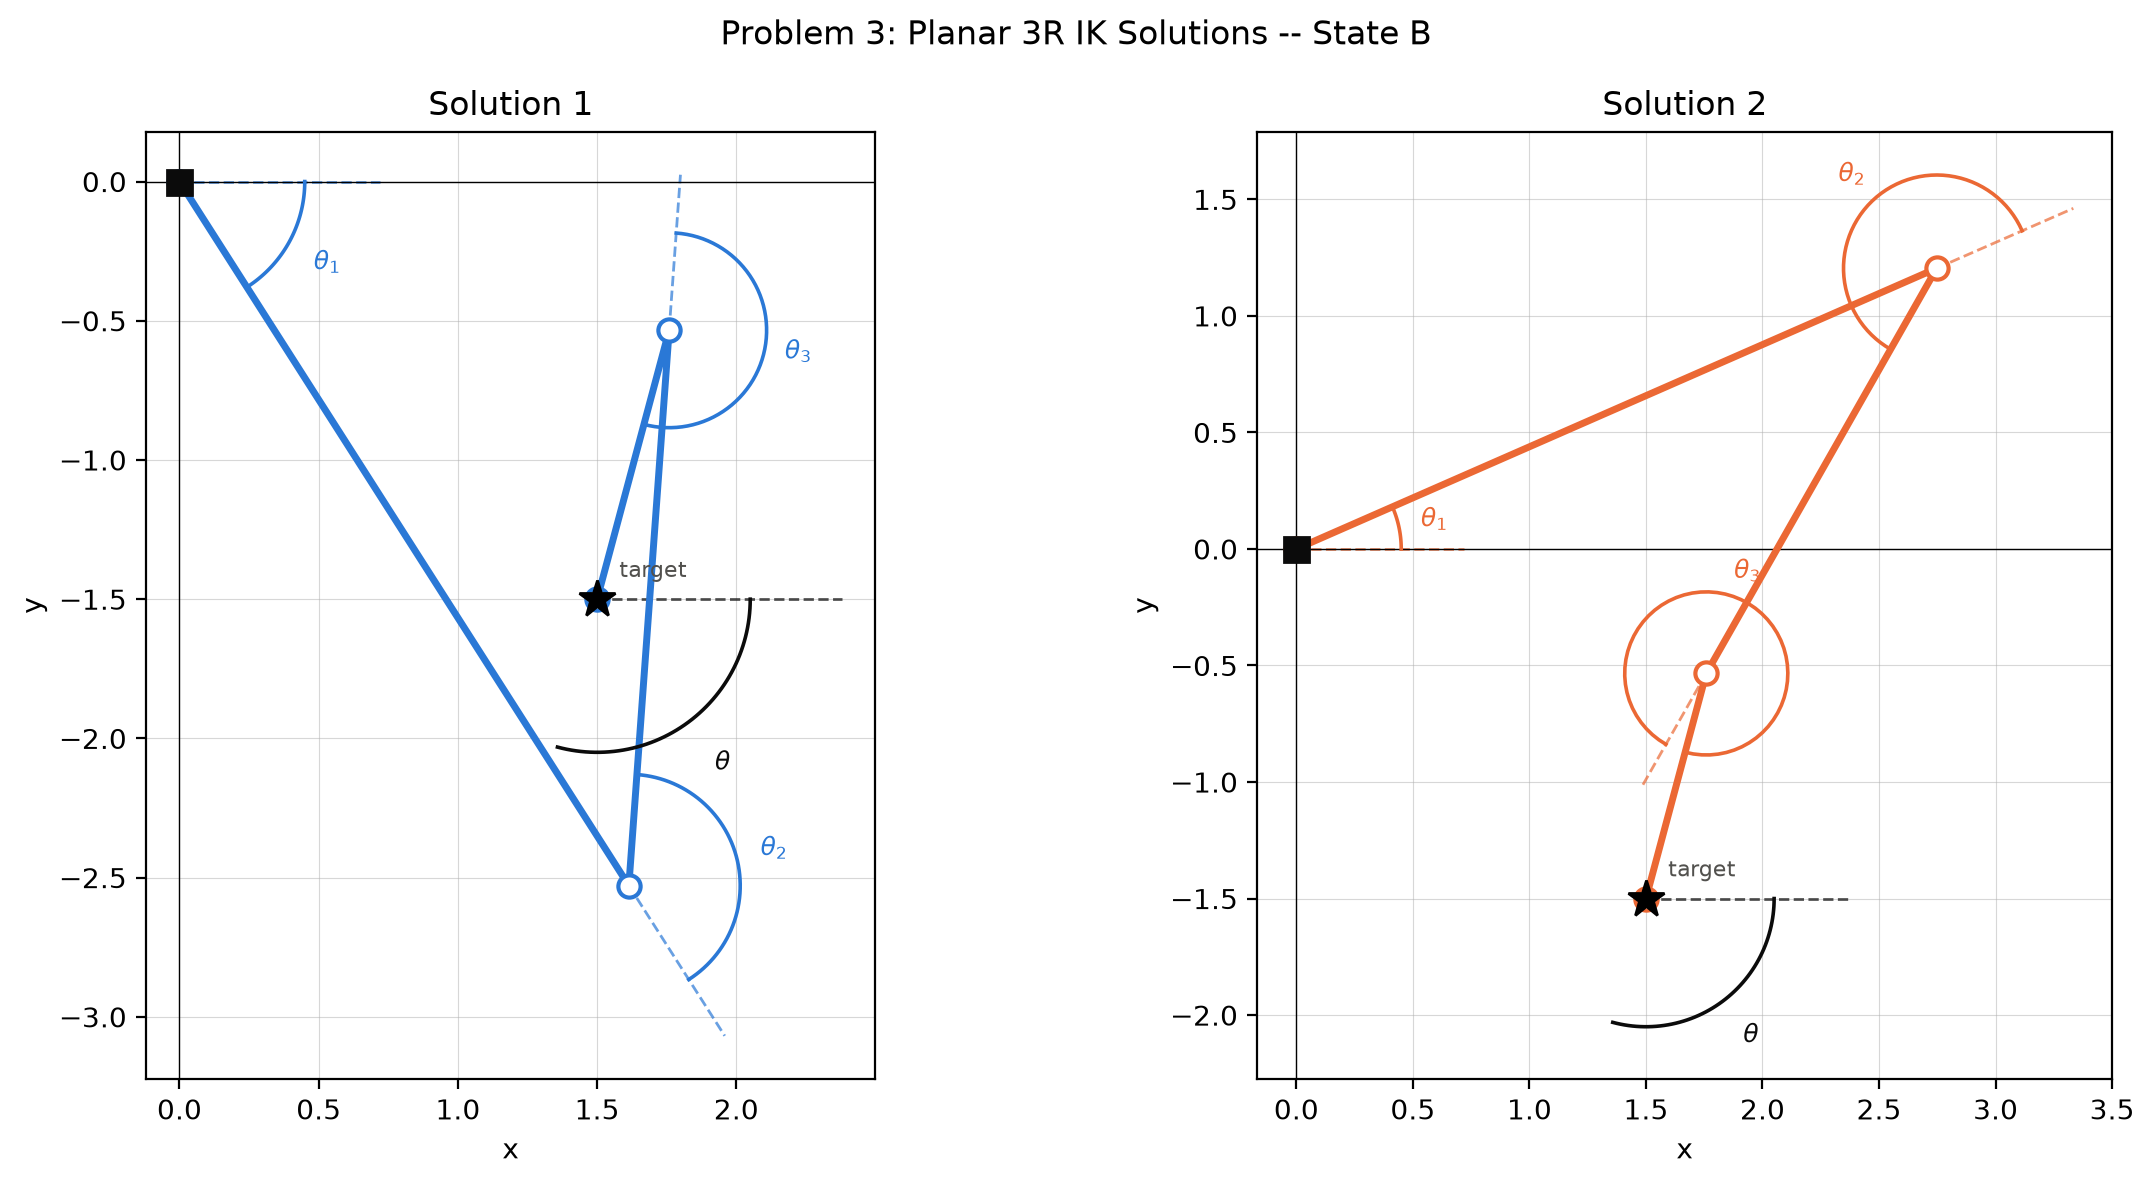
\includegraphics[width=\linewidth]{Figures/Graphs/Problem3_B.png}
    \caption{State B: $(x,y,\theta)=(1.5,\ -1.5,\ -105^\circ)$ -- elbow-up and elbow-down solutions, with joint angles marked at each joint.}
\end{figure}


% ====================================================
% APPENDIX
% ====================================================
\newpage
\appendix
\section*{Appendix: Code Listings}

\subsection*{Problem 3 Code}
\CodeListing{../code/Problem 3.py}{Planar 3R Inverse Kinematics}{lst:p3}

\end{document}
